\documentclass{article}
\usepackage{amsmath}
\usepackage[utf8]{inputenc}
\usepackage{graphicx}
\usepackage{enumerate}
\usepackage{url}
\usepackage{tabto}
\usepackage{pgfplots}
\pgfplotsset{compat=1.12}
\setlength{\parskip}{\baselineskip}%
\setlength{\parindent}{0pt}%

\begin{document}
\begin{titlepage}
\title{Lösning Veckotest 4, MA1439}
\author{Henrik Samuelsson}
\maketitle
\thispagestyle{empty}
\end{titlepage}

\section*{Uppgift 1.}
För vilken exponent $x$ är
\begin{enumerate}[(a)]
\item $3^x \cdot 3^{-2}=\dfrac{3^3}{3}$
\item $7^x + 5 \cdot 7^x = 294$
\end{enumerate}

\textbf{Lösning}
\begin{enumerate}[(a)]
\item $ 3^x \cdot 3^{-2} = \dfrac{3^3}{3} $

$ 3^x \cdot 3^{-2} = 3^2 $

$ 3^x = 3^3 \cdot 3^2 $

$ 3^x = 3^{3 + 2} $

$ 3^x  = 3^5 $

$ x = 5 $
\item $ 7^x + 5 \cdot 7^x = 294 $

$ 7^x(1 + 5) = 294 $

$ 7^x \cdot 6 = 294 $

$ 7^x = 294 / 6 $

$ 7^x = 49 $

$ 7^x = 7 \cdot 7 $

$ 7^x = 7^2 $

$ x = 2 $
\end{enumerate}

\section*{Uppgift 2.}

Lös följande ekvationer exakt. Ge även ett närmevärde med tre decimaler.  
\begin{enumerate}[(a)]
\item $ 6 \cdot 10^x = 24 $
\item $ lg(x) = 4 $
\item $ 4 \cdot lg(1) = x $
\item $ lg(3x) = 5 $
\end{enumerate}

\textbf{Lösning}

\begin{enumerate}[(a)]
\item $ 6 \cdot 10^x = 24 $

$ 10^x = 24 / 6 $

$ 10^x = 4 $

$ x = lg(4) $	\tab(exakt lösning)

$ x = 0,602 $	\tab(närmevärde)

\item $ lg(x) = 4 $

$ x = 10^4 $

$ x = 10000 $	\tab(exakt lösning och närmevärde)

\item $ 4 \cdot lg(1) = x $

$ x = 4 \cdot lg(1) $

$ x = 4 \cdot 0 $

$ x = 0 $	\tab(exakt lösning och närmevärde)

\item $ lg(3x) = 5 $

$ 3x = 10^5 $

$ x = \dfrac{100000}{3} $	\tab(exakt lösning)

$ x = 33333,333$	\tab(närmevärde)

\end{enumerate}
\section*{Uppgift 3.}
Lös ekvationen $ 2^x = 10 $ grafiskt.

\textbf{Lösning}

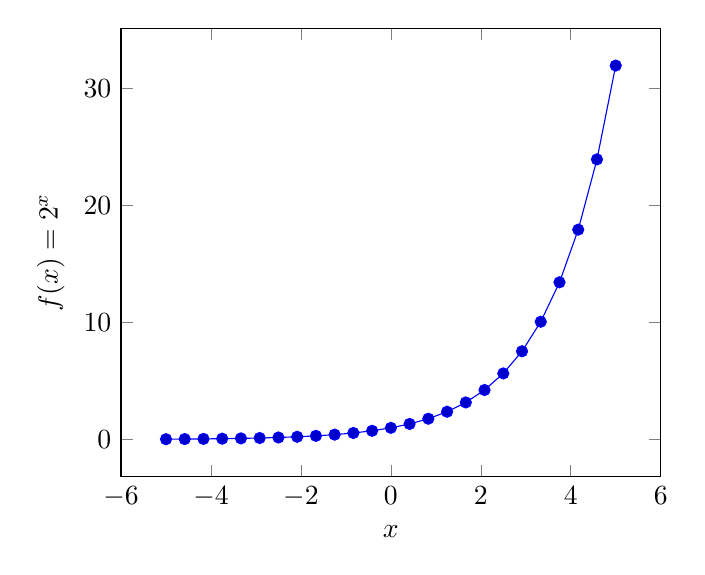
\begin{tikzpicture}
	\begin{axis}[
		xlabel=$x$,
		ylabel={$f(x) = 2^x $}
	]
	% use TeX as calculator:
	\addplot {2^x};
	\end{axis}
\end{tikzpicture} 

\end{document}
